\documentclass[main.tex]{subfiles}

\begin{document}
\maketitle

%\begin{subappendices}
\chapter{Preliminaries}

\section{Quantum Mechanics}
Reference: Chapter 2 of \cite{nielsen2010quantum}

\subsection{Postulates of Quantum Mechanics}

First, we cover the fundamental postulates of quantum mechanics. 

\subsubsection{State Space and State Vector}

Associated with an isolated physical system is a Hilbert space, $\mathcal{H}$. A Hilbert space is a complete inner-product vector space. Note that completeness holds trivially in a finite-dimensional vector space because we have closure with respect to all sequences (and hence any Cauchy sequence in the vector space must converge to a vector in the same space). Nevertheless, the state space of a physical system may be infinite-dimensional. 

A system is completely described by a unit vector $u \in \mathcal{H}$ called the state vector.

For example, consider a system given by a single qubit, which has a two-dimensional state space. Let $\ket{0}$ and $\ket{1}$ be an orthonormal basis for this space. Hence, a state vector in this space is given by 

\begin{align*}
\ket{\psi} = a\ket{0} + b\ket{1}	
\end{align*}


where $a, b \in \CC$ and $|a|^2 + |b|^2 = 1$. 

\subsubsection{Evolution}\label{post-discrete-evol}

The evolution of a closed quantum system is described by a unitary transformation. Recall that an operator $U$ is unitary iff $U^\dagger U = I = UU^\dagger$ (and hence preserves inner products\footnote{and furthermore has a spectral decomposition because it is normal}).

So, let the state of a system at time $t_1$ be given by $\ket{\psi}$ and $\ket{\psi'}$ at $t_2$. Hence,

\begin{align*}
\ket{\psi'} = U\ket{\psi}	
\end{align*}

\subsubsection{Evolution in Continuous Time}\label{post-cts-evol}

Schrodinger's equation provides the time evolution of the state of a quantum system

\begin{align}\label{schro-cts}
i\hbar \frac{d\ket{\psi}}{dt} = H\ket{\psi}	
\end{align}

where $H$ is the (Hermitian) Hamiltonian of the closed system. Because the Hamiltonian is Hermitian it has spectral decomposition 

\begin{align*}
H = \sum_{E} E \ket{E}\bra{E}	
\end{align*}

where $E$ is the energy eigenvalue corresponding to energy eigenstate $\ket{E}$. 

For example, consider the Hamiltonian $H = \hbar \omega X$  (recall that $X = \sigma_X = \begin{pmatrix} 0 & 1 \\ 1 & 0\end{pmatrix}$ from \ref{pauli}). Hence, we solve for its eigenvalues and eigenvectors

\begin{align*}
	\det{ \hbar\omega\begin{pmatrix} -\lambda & 1 \\ 1 & -\lambda\end{pmatrix}} &= 0 \\
	\lambda^2 - 1^2 &= 0 \\
	\lambda &= \pm 1 \\
	\implies E_{\pm} &= \pm \hbar \omega \\
	\hbar\omega\begin{pmatrix} -1 & 1 \\ 1 & -1\end{pmatrix}\ket{E_+} &= 0 \\
	\ket{E_+} &= \frac{1}{\sqrt{2}}\begin{pmatrix}
		1 \\ 1
	\end{pmatrix} \coloneqq \ket{+} \\
	\ket{E_-} &= \ket{-}
\end{align*}

Onwards, notice that we can solve Schrodinger's equation (\ref{schro-cts}) and have

\begin{align*}
	\ket{\psi(t_2)} &= \exp[\frac{-iH(t_2 - t_1)}{\hbar}] \ket{\psi(t_1)}
\end{align*}

and equivalently from \ref{post-discrete-evol} we can represent this transformation with unitary operator $U = \exp[\frac{-iH(t_2 - t_1)}{\hbar}]$. This holds in general and so we can consider the two descriptions from \ref{post-discrete-evol} and \ref{post-cts-evol} interchangeably (the authors prefer the latter). 

\subsubsection{Quantum Measurement}\label{qmeas}

Quantum measurements are described by a collection of measurements operators $\{ M_m \}$ (where the index $m$ refers to the potential measurement outcomes of the experiment) which act on the state space of the system being observed. 

Hence, if the pre-measurement state is $\ket{\psi}$, then 

\begin{align*}
	p(m) = \bra{\psi} M_m^\dagger M_m \ket{\psi}
\end{align*}

and the post-measurement state is 

\begin{align*}
	\frac{M_m \ket{\psi}}{\sqrt{p(m)}}
\end{align*}

Furthermore, $\{ M_m \}$ satisfy the completeness equation

\begin{align*}
\sum_m M_m^\dagger M_m = I
\end{align*}

An important example of a measurement is the measurement of a qubit in the computational basis. This is a measurement of a qubit with two outcomes defined by the measurement operators $M_0 = \ket{0}\bra{0}$ and $M_1 = \ket{1}\bra{1}$.

Now, we see an interesting implication. If we seek to distinguish our physical system from a set of orthogonal states, then we can reliably do so by simply defining each measurement operator to be the outer product of our states of interest. We add a final operator defined to be the remaining complement of the identity in order to satisfy the completeness equation. 

On the flipside, two non-orthogonal states $\ket{\psi_1}$ and $\ket{\psi_2}$ necessarily share a parallel component in their orthogonal decomposition. Hence, a measurement outcome that corresponds to the pre-measurement state being $\ket{\psi_1}$ with probability $p = 1$ has a probability $p'>0$ of having been in state $\ket{\psi_2}$. 

\subsubsection{Projective Measurements}

There exists a special class of quantum measurements known as projective measurements. These measurements can be described by an observable $M$, a hermitian operator on the state space being observed. $M$ has spectral decomposition

\begin{align*}
M = \sum_m m P_m	
\end{align*}

where $P_m$ is the projector onto the eigenspace of $M$ with eigenvalues $m$. 

Furthermore, if the pre-measurement state is $\ket{\psi}$, then 

\begin{align*}
p(m) = 	\bra{\psi} P_m \ket{\psi}
\end{align*}

and the post-measurement state is 

\begin{align*}
	\frac{P_m \ket{\psi}}{\sqrt{p(m)}}
\end{align*}

This simplifies the formula for the expected value of a measurement

\begin{align*}
\langle M \rangle &= \sum_m m p(m) \\
&= \bra{\psi} (\sum_m m P_m)  \ket{\psi} \\
&= 	\bra{\psi} M \ket{\psi}
\end{align*}

For example, consider projective measurements on the system given by single qubits with observable Pauli matrix $Z$. Hence, $Z$ has eigenvalues $+1$ and $-1$ and eigenstates $\ket{0}$ and $\ket{1}$, respectively. So, consider state $\ket{\psi} = \frac{\ket{0} + \ket{1}}{\sqrt{2}}= \ket{+}$ $\implies$ $p(+1) = \bra{+}\ket{0}\bra{0}\ket{+} = \frac{1}{2}$. Similarly, $p(-1) = \frac{1}{2}$. 

More generally, suppose $v$ is an arbitrary 3-d vector. We can define an observable

\begin{align*}
v \cdot \sigma = v_1\sigma_x + v_2 \sigma_y + v_3\sigma_z
\end{align*}

\begin{example}
Suppose we have a qubit in the state $\ket{0}$, and we measure the observable $X$. What is the average value of $X$? What is the standard deviation of $X$?
	
	\begin{proof}
		$X$ has eigenvalues $+1$ and $-1$ and eigenstates $\ket{+}$ and $\ket{-}$, respectively. Hence,
		
	\begin{align*}
	\< X \> &= \bra{\psi} X 	\ket{\psi} \\
	&= \bra{\psi} (\ket{+}\bra{+} - \ket{-}\bra{-}) \ket{\psi} \\
	&= \bra{0}\ket{+}\bra{+}\ket{0} - \bra{0}\ket{-}\bra{-}\ket{0}\\
	&= \frac{1}{2} - \frac{1}{2} = 0
	\end{align*}
	
	Furthermore,

	\begin{align*}
	\< M^2 \> - \< M \>^2 &= \bra{\psi} M^2 	\ket{\psi} - 0 \\
	&= \bra{\psi} (\ket{+}\bra{+} + \ket{-}\bra{-}) \ket{\psi} \\
	&= \frac{1}{2} + \frac{1}{2} = 1
	\end{align*}
	\end{proof}
	
\end{example}

\begin{proposition}
$v \cdot \sigma$ has eigenvalues $\pm 1$ and the projectors onto the corresponding eigenspaces are given by $P_{\pm} = (I \pm v \cdot \sigma)/2$.

\begin{proof}
	First, $v\cdot \sigma$ is Hermitian so it's spectral decomposition is given by $v \cdot \sigma = U \Lambda U^\dag$ for some unitary $U$, diagonal matrix $\Lambda$. Hence, using $(v\cdot \sigma)^2 = I$ we have
	
	\begin{align*}
		I &= (v \cdot \sigma)^2 = (U \Lambda U^\dag)^2 \\
		&= U \Lambda^2 U^\dag \\
		\implies U^\dag I U &= \Lambda^2 \\
		I & = \Lambda^2
	\end{align*}

Therefore, $\Lambda$ must have diagonal entries $\pm 1$. 

Next, $P_i P_j = \delta_{ij}P_j$ since if $i \neq j$ then $(I + v \cdot \sigma)(I - v\cdot \sigma) = I - (v \cdot \sigma)^2 = I - I = 0$. Furthermore, $P_+ + P_- = (I + v \cdot \sigma)/2 + (I - v \cdot \sigma)/2 = I$. 

Finally, $(+1)P_+ + (-1)P_- = (I + v \cdot \sigma)/2 - (I - v \cdot \sigma)/2 = v \cdot \sigma$. 
\end{proof}
\end{proposition}

\subsubsection{POVM measurements}\label{povm}

POVMs are best viewed as a special case of the general measurement formalism, providing the simplest means to study post-measurement statistics without knowledge of the post measurement state.

From above, $p(m) = \bra{\psi} M_m^\dagger M_m \ket{\psi}$ so if we define $E_m \coloneqq M_m^\dagger M_m$ (which is hence positive from \ref{posop}) then these $E_m$'s are sufficient for the purpose of computing probabilities. We denote $\{ E_m \}$ as a POVM. POVMs also satisfy the completeness relation.

Note that projective operators are the special case of being equivalent to their respective POVM element because $E_m = P_m^\dag P_m = P_m$. 

\begin{proposition}
Any measurement where the measurement operators and the POVM elements coincide is a projective measurement

\begin{proof}
We would then have $M_m = E_m = M_m^\dag M_m$. Furthermore, $E_m$ is a positive operator $\implies$ $M_m = M_m^\dag M_m = M_m M_m^\dag = M_m^\dag$ so $M_m$ is Hermitian. Hence, $M_m = M_m^2$ so the measurement is projective.
\end{proof}	
\end{proposition}

Nevertheless, the POVM formalism is a useful guide in for our intuition in quantum information. Consider if Alice prepares some state for Bob that is either $\ket{\psi_1} = \ket{0}$ or $\ket{\psi_2} = \frac{\ket{0} + \ket{1}}{\sqrt{2}}$. Recall from \ref{qmeas}, Bob can't determine which state was prepared with full certainty (because of the shared orthogonal component $\ket{0}$). Still, we can define a POVM\footnote{verify that completeness and these being positive operators holds}

\begin{align*}
E_1 &= \frac{\sqrt{2}}{1+\sqrt{2}}\ket{1}\bra{1}	\\
E_2 &= \frac{\sqrt{2}}{1+\sqrt{2}}\frac{(\ket{0} - \ket{1})(\bra{0} - \bra{1})}{2} \\
E_3 &= I - E_1 - E_2
\end{align*}

Now, notice what happens. 

\begin{align*}
\bra{\psi_1} E_1 \ket{\psi_1} &= \bra{0} \frac{\sqrt{2}}{1+\sqrt{2}}\ket{1}\bra{1}\ket{0} \\
	&= 0 \\
\bra{\psi_2} E_1 \ket{\psi_2} &= \frac{\bra{0} + \bra{1}}{\sqrt{2}}\frac{\sqrt{2}}{1+\sqrt{2}}\ket{1}\bra{1}\frac{\ket{0} + \ket{1}}{\sqrt{2}} \\
	&= \frac{\sqrt{2}}{2\sqrt{2} + 2} > 0 
\end{align*}

Hence, if we observe $E_1$ after the measurement described by $\{ E_1, E_2, E_3 \}$, then Alice must've prepared $\ket{\psi_2}$. Similarly,

\begin{align*}
\bra{\psi_1} E_2 \ket{\psi_1} &= \bra{0} \frac{\sqrt{2}}{1+\sqrt{2}}\frac{(\ket{0} - \ket{1})(\bra{0} - \bra{1})}{2}\ket{0} \\
	&= \frac{\sqrt{2}}{2\sqrt{2} + 2} > 0 \\
\bra{\psi_2} E_2 \ket{\psi_2} &= \frac{\bra{0} + \bra{1}}{\sqrt{2}}\frac{\sqrt{2}}{1+\sqrt{2}}\frac{(\ket{0} - \ket{1})(\bra{0} - \bra{1})}{2}\frac{\ket{0} + \ket{1}}{\sqrt{2}} \\
	&= 0
\end{align*}

so if we observe $E_2$, then Bob concludes that Alice prepared $\ket{\psi_1}$. Our routine is imperfect because we may observe $E_3$ and hence would infer nothing of the original state. Still, we would never $\textit{incorrectly}$ guess given that we allow ourselves to abstain when we see $E_3$. 

\begin{proposition} Suppose Bob is given a quantum state chosen from a set $S = \ket{\psi_1} , \cdots , \ket{\psi_m}$ of linearly independent states. Construct a POVM $\{ E_1 , \cdots , E_{m+1} \}$ such that if outcome $E_i$ occurs, $1 \leq i \leq m$, then Bob knows with certainty that he was given state $\ket{\psi_i}$.

\begin{proof}
	To distinguish the states we require $\bra{\psi_i} E_j \ket{\psi_i} = p_i \delta_{ij}$ where $p_i > 0$ and $1 \leq i,j \leq m$. 

So, we can use the Gram-Schmidt process using $S$ as our linearly independent set. This will give us an orthonormal set $U = \ket{\phi_1} , \cdots , \ket{\phi_m}$ that spans the same subspace as $S$. Next, we can represent each $\ket{\psi_i}$ in this orthonormal basis, $U$. Finally, for each $i$ we can find a vector $\ket{\psi'_i}$ in the span of $U$ that is orthogonal to all $\ket{\psi_j}, j \neq i$. Hence, we can define $E_i = \ket{\psi_i'} \bra{\psi_i'}, 1 \leq i \leq m$. Finally, take $E_{m+1} = I - \sum_m E_i$. 

Creating an optimal POVM is much trickier (in the sense of minimizing the probability $p_{m+1}$).
\end{proof}
\end{proposition}

From this Proposition, we see that POVMs present a reliable way to distinguish non-orthogonal (but linearly independent) states given that we allow for the slack of an "inconclusive" measurement ($E_{m+1}$). 

\subsubsection{Composite Systems}

The state space of a composite physical system is the tensor product of the state spaces of the component physical systems. 
 
Interestingly, we can show that a general quantum measurement (as described in \ref{qmeas}) can be implemented as a projective measurement coupled with unitary dynamics.

Consider a quantum system with state space $Q$ and measurements $M_m$ on this system. We can introduce an \textit{ancilla} system $M$ with orthonormal basis $\ket{m}$ which is in one-to-one correspondence with the possible outcomes of the measurement we wish to implement. 

So, let $\ket{0}$ be a fixed state of $M$ and define an operator $U$ on $\ket{\psi}\ket{0}$ (with $\ket{\psi}$ as a state of $Q$) by

\begin{align*}
U\ket{\psi}\ket{0} \coloneqq \sum_m M_m \ket{\psi}\ket{m}
\end{align*}

Hence,

\begin{align*}
\bra{\phi}\bra{0}U^\dag U \ket{\psi}	 \ket{0} &= \sum_m \sum_{m'} \bra{\phi} M_m^\dag M_{m'} \ket{\psi}\bra{m}\ket{m'} \\
\intertext{So, because the states $\ket{m}$ are orthonormal}
&= \sum_m\bra{\phi} M_m^\dag M_{m} \ket{\psi} \\
\intertext{and finally by the completeness of $M_m$}
&= \bra{\phi}\ket{\psi}
\end{align*}

This tells us that $U$ preserves inner products between states of the form $\ket{\psi}\ket{0}$. Furthermore, we can show that $U$ can be extended to a unitary operator on $Q \otimes M$ (exercise).

Hence, consider a projective measurement on the two systems ($U\ket{\psi}\ket{0}$) given by projectors $P_m \coloneqq I_Q \otimes \ket{m}\bra{m}$. So,

\begin{align*}
p(m) &= \bra{\psi} \bra{0} U^\dag P_m U \ket{\psi} \ket{0} \\
&= \sum_{m'}\sum_{m''} \bra{\psi} M_{m'}^\dag \bra{m'} (I_Q \otimes \ket{m}\bra{m})M_{m''} \ket{\psi} \ket{m''} \\
&= \bra{\psi} M_m^\dag M_m \ket{\psi}
\end{align*}

which agrees with the general result from \ref{qmeas}. Similarly, the post-measurement state is as expected. Hence, we've shown that unitary dynamics, projective measurements, and ancillary systems can be used together to describe any general measurement.

A state of a composite system having this property is said to be entangled. 

\subsection{Superdense Coding}

Suppose Alice is in possession of two classical bits of information she wishes to transmit to Bob, but is only allowed to send a single qubit to Bob.

 Now, suppose that Alice and Bob initially share a pair of qubits in the entangled state from above
 
\begin{align*}
\ket{\psi} = \frac{\ket{00} + \ket{11}}{\sqrt{2}}	
\end{align*}
 
 where Alice is initially holding the first qubit and Bob the second. She can then apply a particular gate to send a bit string. Below shows the corresponding gate and resulting state
 
 \begin{table}[H]
 	\begin{center}
 \begin{tabular}{l | c | l }
 	Bit String & Applied gate  & Resulting state\\
 	\hline 
 	00 & -- & $\frac{\ket{00} + \ket{11}}{\sqrt{2}}$\\
 	01 & Z & $\frac{\ket{00} - \ket{11}}{\sqrt{2}}$\\
 	10 & X & $\frac{\ket{10} + \ket{01}}{\sqrt{2}}$\\
 	11 & iY & $\frac{-\ket{10} + \ket{01}}{\sqrt{2}}$
 \end{tabular}
 \end{center}
 \end{table}

Observe that these are the Bell states (see \ref{bellstates}). Furthermore, Bell states form an orthonormal basis and hence can be distinguished (as we've discussed in \ref{povm}). Hence, Alice needs only to interact with the single qubit to transmit two classical bits of information to Bob.

\subsection{The Density Operator}

An alternative formulation of quantum mechanics is possible using a tool known as the density operator. 

Suppose a quantum system is one of a number of states $\ket{\psi}$ with probability $p_i$. We call $\{p_i, \ket{\psi_i} \}$ an ensemble of pure states. The density operator is defined

\begin{align*}
\rho \coloneqq \sum_i p_i \ket{\psi_i}\bra{\psi_i}	
\end{align*}

Evolution of the density operator (under a unitary transformation) can be derived readily

\begin{align*}
\sum_i p_i U\ket{\psi_i}\bra{\psi_i}U^\dag = U\rho U^\dag	
\end{align*}

If we perform a measurement with operator $M_m$ with initial state $\ket{\psi_i}$ then

\begin{align*}
p(m\mid i) &= \bra{\psi_i} M_m^\dag M_m \ket{\psi_i} \\
&= \tr(M_m^\dag M_m \ket{\psi_i}\bra{\psi_i})
\end{align*}

using \ref{trop}. 

Hence, summing this conditional probability across all initial states we have

\begin{align*}
	p(m) &= \sum_i p_i \tr(M_m^\dag M_m \ket{\psi_i}\bra{\psi_i}) \\
	&= \tr(M_m^\dag M_m \rho)
\end{align*}

The state after obtaining measurement result $m$ on initial state $\ket{\psi_i}$ is

\begin{align*}
\ket{\psi_i^m} = \frac{M_m \ket{\psi_i}}{\sqrt{\bra{\psi_i}M_m^\dag M_m\ket{\psi_i}}}	
\end{align*}

and so the density operator after result $m$ is given by

\begin{align*}
	\rho_m &= \sum_i p(i \mid m ) \ket{\psi_i^m} \bra{\psi_i^m} \\
	&= \sum_i p(i \mid m )\frac{M_m \ket{\psi_i}\bra{\psi_i}M_m^\dag}{\bra{\psi_i}M_m^\dag M_m\ket{\psi_i}}
\end{align*}

Furthermore, from Bayes' rule we have that $p(i \mid m) = \frac{p(m \mid i)p(i)}{p(m)}$ so we can simplify

\begin{align*}
	\rho_m &= \sum_i \frac{p(m \mid i)p(i)}{p(m)}\frac{M_m \ket{\psi_i}\bra{\psi_i}M_m^\dag}{\bra{\psi_i}M_m^\dag M_m\ket{\psi_i}} \\
	&= \sum_i \frac{p(i)\bra{\psi_i} M_m^\dag M_m \ket{\psi_i}}{\tr(M_m^\dag M_m \rho)}\frac{M_m \ket{\psi_i}\bra{\psi_i}M_m^\dag}{\bra{\psi_i}M_m^\dag M_m\ket{\psi_i}} \\
	&= \sum_i \frac{p(i)M_m \ket{\psi_i}\bra{\psi_i}M_m^\dag}{\tr(M_m^\dag M_m \rho)} \\
	&= \frac{M_m\rho M_m^\dag}{\tr(M_m^\dag M_m \rho)}
\end{align*}

A quantum state whose state $\ket{\psi}$ is known exactly is said to be in a pure state. In this case the density operator is simply $\rho = \ket{\psi}\bra{\psi}$. Otherwise, $\rho$ is in a mixed state.

A pure state satisfies $\tr(\rho^2) = 1$ and a mixed state $\tr(\rho^2) < 1$.

Imagine that our record of the result $m$ of a measurement was lost. We would have a quantum system in the state $\rho_m$ with probability $p(m)$ without knowing the actual value of $m$. Hence, the system would be described as

\begin{align*}
\rho &= \sum_m p(m) \rho_m	\\
&= \sum_m M_m \rho M_m^\dag 
\end{align*}

We may wish to move away from the interpretation of the density operator as a means of describing ensembles of quantum states.

\begin{theorem}
An operator $\rho$ is a density operator associated to some ensemble $\{p_i, \ket{\psi_i}\}$ if and only if it satisfies the conditions

\begin{enumerate}
\item $\rho$ has trace equal to one
\item $\rho$ is a positive operator	
\end{enumerate}

\begin{proof}
	We show one direction (see the text for the other). Let $\rho$ be a density operator. Hence,
	
	\begin{align*}
	\tr(\rho) &= \sum_i p_i \tr(\ket{\psi_i}\bra{\psi_i}) \\
	&= 	\sum_i p_i =1
	\end{align*}

because $\tr(\ket{\psi_i}\bra{\psi_i}) = \psi_{i, 11}^2 + \psi_{i, 22}^2 + \cdots \psi_{i, nn}^2 = 1$ by normalization. 

Furthermore, suppose $\ket{\phi}$ resides in the vector space

\begin{align*}
\bra{\phi} \rho \ket{\phi} &= \sum_i p_i \bra{\phi}\ket{\psi_i}\bra{\psi_i}\ket{\phi} \\
&= \sum_i p_i |\bra{\phi}\ket{\psi_i}|^2 \geq 0
\end{align*}
so we have positivity.
\end{proof}	
\end{theorem}

The use of this theorem is that we can define a density operator to be a positive operator with trace one and hence reformulate the postulates of quantum mechanics without speaking of ensembles.

This reformulation shines when describing quantum systems whose state is not known and when describing subsystems a composite quantum system.

\begin{proposition}
Let $\rho$ be a density operator. $\tr(\rho^2) \leq 1$ with equality iff $\rho$ is a pure state.
\begin{proof}
\begin{align*}
\rho^2 &= \sum_i p_i \ket{\psi_i}\bra{\psi_i}	\sum_{i'} p_{i'} \ket{\psi_{i'}}\bra{\psi_{i'}}	\\
&= 	\sum_i p_i^2 \ket{\psi_i}\bra{\psi_i}
\end{align*}

by orthonormality. Hence,

\begin{align*}
\tr \rho^2 &= \sum_i \sum_j p_i^2 \psi_{i,jj}^2 \\
\intertext{And $\sum_j \psi_{i,jj}^2=1$ by normalization}
&= \sum_i p_i^2
\end{align*}

Now, we have that $\sum_i p_i = 1 \implies \sum_i p_i^2 = 1 \iff p_i = 1$. If $p_i = 1$, then there is only one index and hence we have a pure state. Otherwise, $\sum_i p_i^2 < 1$ and we have a mixed state.
\end{proof}	
\end{proposition}

Remember that different ensembles of quantum states can give rise to a specific density matrix and hence one must avoid assuming that the eigenvectors and eigenvalues have special significance with regard to the represented ensemble of quantum states.

Nevertheless, there is value in discussing which ensembles give rise to the same density matrix (notably in quantum noise and error correction). Let $\ket{\tilde{\psi_i}}$ generate $\rho$ i.e. $\rho\coloneqq\sum_i\ket{\tilde{\psi_i}}\bra{\tilde{\psi_i}}$. Note that $\ket{\tilde{\psi_i}} = \sqrt{p_i}\ket{\psi_i}$ is clearly not necessarily normalized. Now, we have the following theorem.

\begin{theorem}
The sets $\ket{\tilde{\psi_i}}$ and $\ket{\tilde{\phi_j}}$ generate the same $\rho$ if and only if

\begin{align*}
	\ket{\tilde{\psi_i}} = \sum_j u_{ij}\ket{\tilde{\phi_j}}
\end{align*}

where the matrix with matrix elements $u_{ij}$ is unitary.
\begin{proof}
	See the text.
\end{proof}
\end{theorem}

As mentioned above, density operators are powerful tools for describing subsystems of composite systems. 
 
Suppose we have physical systems $A$ and $B$, whose state is described by $\rho^{AB}$. The reduced density operator for system $A$ is defined by

\begin{align*}
\rho^A \coloneqq \tr_B(\rho^{AB})
\end{align*}

where $\tr_B$ is a map of operators known as the partial trace over system $B$ which is defined by

\begin{align*}
\tr_B(\ket{a_1}\bra{a_2} \otimes \ket{b_1}\bra{b_2}) &= \ket{a_1}\bra{a_2} \tr( \ket{b_1}\bra{b_2}) \\
&= \ket{a_1}\bra{a_2} \bra{b_2}\ket{b_1}
\end{align*}

Hence, consider the Bell state $\frac{\ket{00} + \ket{11}}{\sqrt{2}}$ and the reduced density operator of its first qubit

\begin{align*}
\rho &= \frac{\ket{00} + \ket{11}}{\sqrt{2}}\frac{\bra{00} + \bra{11}}{\sqrt{2}} \\
\rho^1 &= \frac{\ket{0}\bra{0}\bra{0}\ket{0}+\ket{1}\bra{0}\bra{0}\ket{1}+ \ket{0}\bra{1}\bra{1}\ket{0}+ \ket{1}\bra{1}\bra{1}\ket{1}}{2} \\
&= \frac{\ket{0}\bra{0} + \ket{1}\bra{1}}{2} \\
&= \frac{I}{2}
\end{align*}

Oddly, $\tr(\frac{I^2}{4}) = 1/2 < 1$ so the first qubit is in a mixed state despite the system as a whole being in a pure state. This is another hallmark of quantum entanglement. 

\begin{example}
For each of the four Bell states, we can find the reduced density operator for each qubit
\end{example}

First, $\frac{\ket{00} + \ket{11}}{\sqrt{2}}$

\begin{align*}
\rho &= \frac{\ket{00} + \ket{11}}{\sqrt{2}}\frac{\bra{00} + \bra{11}}{\sqrt{2}} \\
\rho^1 &= \frac{\ket{0}\bra{0}\bra{0}\ket{0}+\ket{1}\bra{0}\bra{0}\ket{1}+ \ket{0}\bra{1}\bra{1}\ket{0}+ \ket{1}\bra{1}\bra{1}\ket{1}}{2} \\
&= \frac{\ket{0}\bra{0} + \ket{1}\bra{1}}{2} = \frac{I}{2} \\
\rho^2 &= \frac{\ket{0}\bra{0}\bra{0}\ket{0}+\ket{1}\bra{0}\bra{0}\ket{1}+ \ket{0}\bra{1}\bra{1}\ket{0}+ \ket{1}\bra{1}\bra{1}\ket{1}}{2} \\
&= \frac{\ket{0}\bra{0} + \ket{1}\bra{1}}{2} = \frac{I}{2}
\end{align*}

The remaining three are similar.
%$\frac{\ket{10} + \ket{01} }{\sqrt{2}}$
%$\frac{\ket{01} - \ket{10} }{\sqrt{2}}$

\subsection{Quantum Teleportation}
Quantum teleportation is a procedure for sending quantum information from Alice to Bob, given that Alice and Bob share an EPR pair, and have a classic communications channel. Recall that the need for Alice to communicate her result to Bob prevents faster than light communication.

The state to be teleported is $\ket{\psi} = \alpha\ket{0} + \beta\ket{1}$. We can use the circuit shown in the figure below to perform this telerportation, with inputs $\ket{\psi} \ket{\beta_{00}}$ where $\ket{\beta_{00}}$ is the Bell state $\frac{\ket{00} + \ket{11} }{\sqrt{2}}$. Hence,

\begin{align*}
	\ket{\psi} \ket{\beta_{00}} &= \frac{1}{\sqrt{2}}\Big[\alpha\ket{0}(\ket{00} + \ket{11}) + \beta\ket{1}(\ket{00} + \ket{11})\Big]
\end{align*}


\begin{figure}[H]
\centering
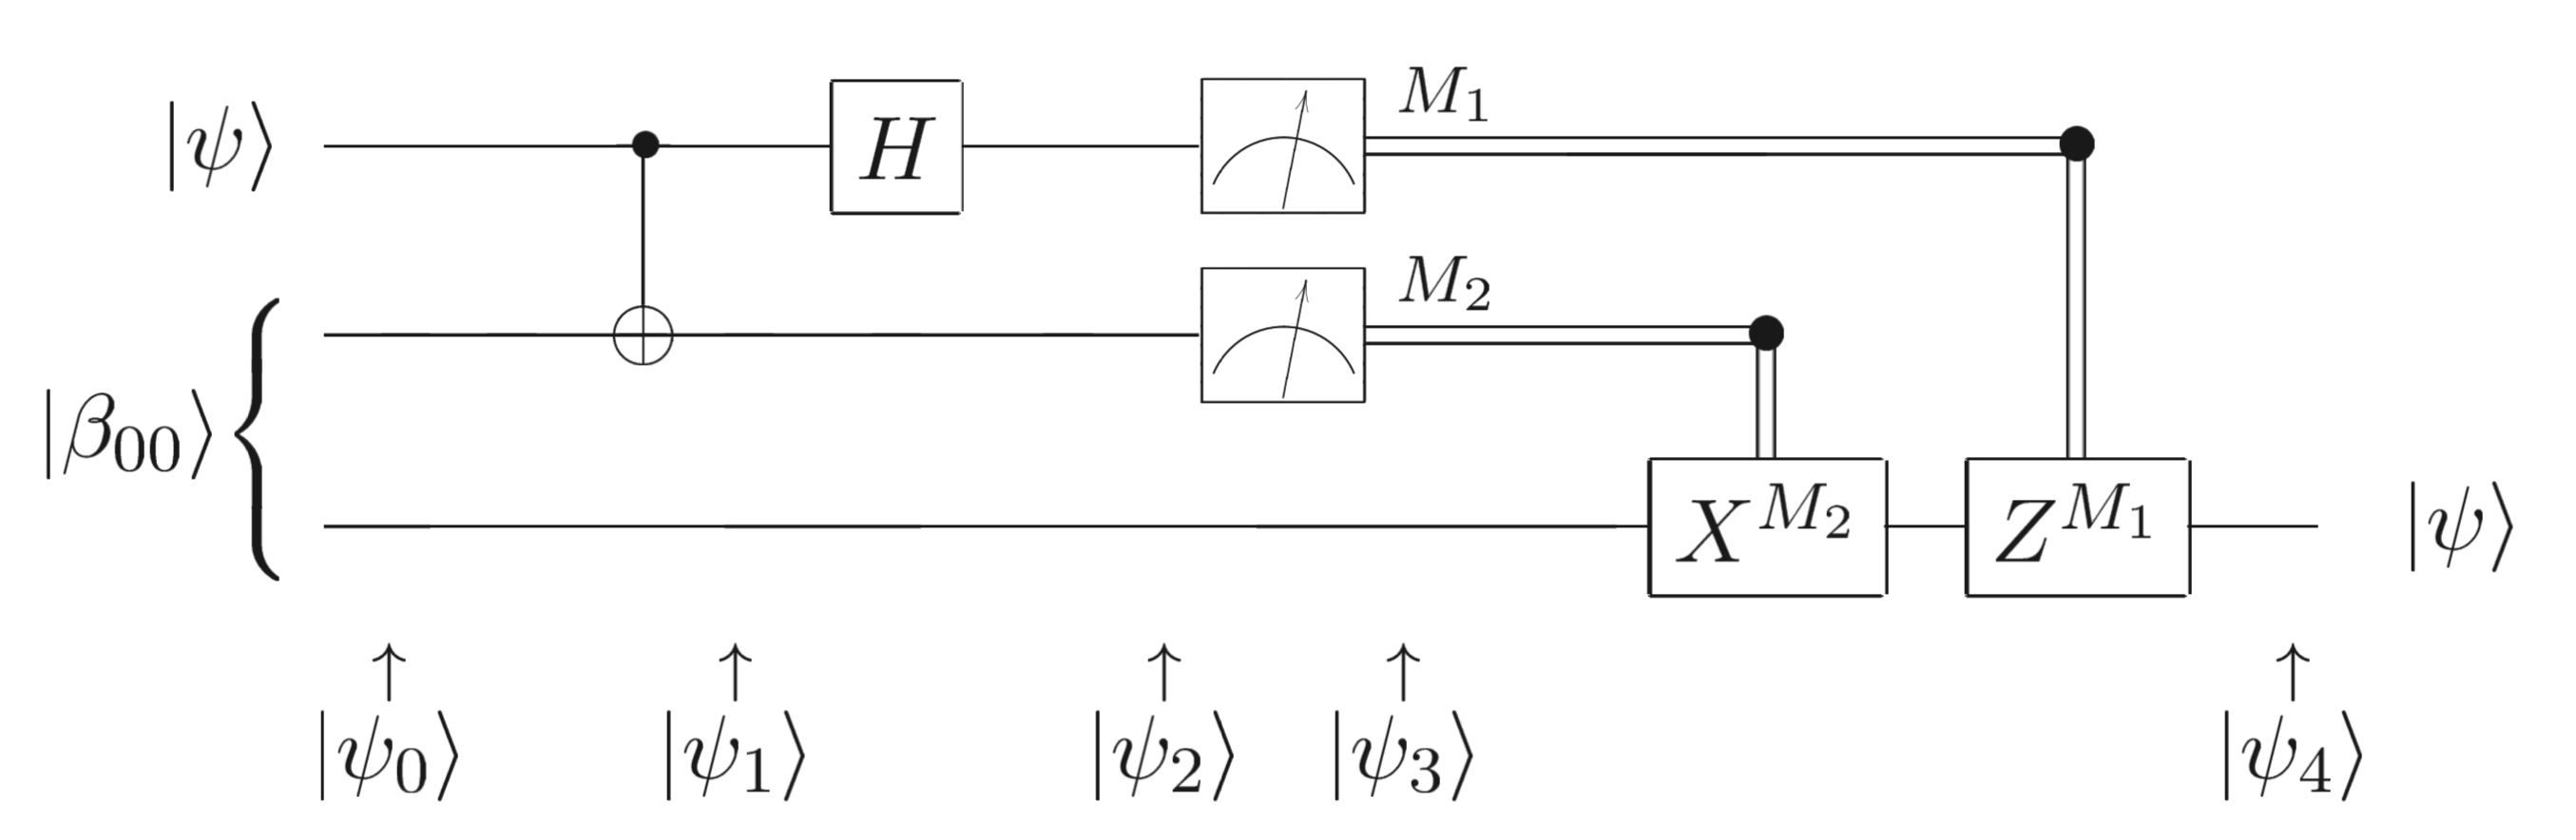
\includegraphics[width=\linewidth]{images/teleportation_circuit.png}	
\caption{Two top lines are Alice's system and bottom is Bob's}
\end{figure}

Recall the controlled-\texttt{NOT} (\texttt{CNOT}) takes $\ket{a}\ket{b}$ to $\ket{a}\ket{b \oplus a}$. The other gates in the circuit are summarized in the diagram below.

\begin{figure}[H]
\centering
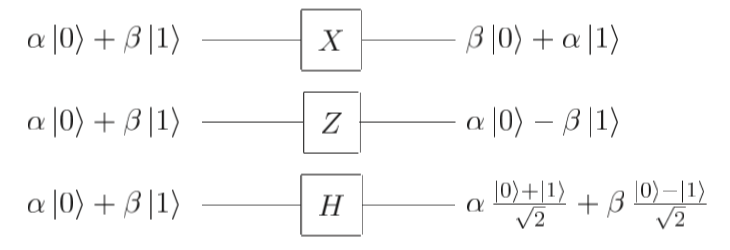
\includegraphics[width=0.5\linewidth]{images/basic_gates.png}	
\caption{Basic gates}
\end{figure}

So, the first two qubits belong to Alice and the third to Bob. Alice sends her qubits through a \texttt{CNOT} obtaining

\begin{align*}
\ket{\psi_1} &= \frac{1}{\sqrt{2}}\Big[\alpha\ket{0}(\ket{00} + \ket{11}) + \beta\ket{1}(\ket{10} + \ket{01})\Big]
\end{align*}

Then, Alice's first qubit is sent through a Hadamard gate which gives

\begin{align*}
\ket{\psi_2} &= \frac{1}{2}\Big[\alpha(\ket{0}+\ket{1})(\ket{00} + \ket{11}) + \beta(\ket{0}-\ket{1})(\ket{10} + \ket{01})\Big] \\
&= \frac{1}{2}\Big[ \ket{00} (\alpha\ket{0} + \beta\ket{1}) + \ket{01}(\alpha\ket{1} + \beta \ket{0}) + \ket{10}(\alpha\ket{0} - \beta\ket{1}) + \ket{11}(\alpha\ket{1} - \beta\ket{0}) \Big]
\end{align*}

Now, observe that each grouping in this expression has Alice's bits in a different state ($\ket{00},\ket{01},\ket{10},\ket{11}$), each of which Alice may observe after a measurement. Curiously, each of these groupings has a unique corresponding state for Bob's qubits. Hence, we know the state of Bob's qubits given knowledge of the outcome of Alice's measurement.

Furthermore, note that each of the possible states of Bob's qubits after Alice's measurements can be readily transformed to $\ket{\psi}$. Consider the four cases

\begin{enumerate}
\item Alice measures $00$. Hence, Bob's state is already $\ket{\psi}$. 
\item Alice measures $01$. Hence, Bob's state is $\alpha\ket{1} + \beta \ket{0}$. So, just apply the $X$ gate. 
\item Alice measures $10$. Hence, Bob's state is $\alpha\ket{0} - \beta\ket{1}$. So, just apply the $Z$ gate to flip the second sign. 
\item Alice measures $11$. Hence, Bob's state is $\alpha\ket{1} - \beta\ket{0}$. So, apply the $X$ gate to flip the bits, then the $Z$ gate to flip the second sign. 
\end{enumerate}

So that's what the notation in the circuit above means, we apply $X$ or $Z$ to Bob's qubits to recover $\ket{\psi}$ depending on the outcome of Alice's measurement.

Pretty cool, right? Let's look at this a level deeper using the density operator formalism we've developed. Each of the 4 cases have probability $\frac{1}{4}$ of occurring after the measurement. Hence, the density operator is given by

\begin{align*}
	\rho =& \frac{1}{4}\Big[ \ket{00}\bra{00} (\alpha\ket{0} + \beta\ket{1})(\alpha^*\bra{0} + \beta^*\bra{1}) + \ket{01}\bra{01}(\alpha\ket{1} + \beta \ket{0})(\alpha^*\bra{1} + \beta^* \bra{0}) \\
	&+ \ket{10}\bra{10}(\alpha\ket{0} - \beta\ket{1})(\alpha^*\bra{0} - \beta^*\bra{1}) + \ket{11}\bra{11}(\alpha\ket{1} - \beta\ket{0})(\alpha^*\bra{1} - \beta^*\bra{0}) \Big]
\end{align*}

So, the reduced density operator of Bob's system is

\begin{align*}
	\rho^B =& \frac{1}{4}\Big[ \bra{00}\ket{00} (\alpha\ket{0} + \beta\ket{1})(\alpha^*\bra{0} + \beta^*\bra{1}) + \bra{01}\ket{01}(\alpha\ket{1} + \beta \ket{0})(\alpha^*\bra{1} + \beta^* \bra{0}) \\
	&+ \bra{10}\ket{10}(\alpha\ket{0} - \beta\ket{1})(\alpha^*\bra{0} - \beta^*\bra{1}) + \bra{11}\ket{11}(\alpha\ket{1} - \beta\ket{0})(\alpha^*\bra{1} - \beta^*\bra{0}) \Big] \\
	=& \frac{1}{4}\Big[(\alpha\ket{0} + \beta\ket{1})(\alpha^*\bra{0} + \beta^*\bra{1}) + (\alpha\ket{1} + \beta \ket{0})(\alpha^*\bra{1} + \beta^* \bra{0}) \\
	&+ (\alpha\ket{0} - \beta\ket{1})(\alpha^*\bra{0} - \beta^*\bra{1}) + (\alpha\ket{1} - \beta\ket{0})(\alpha^*\bra{1} - \beta^*\bra{0}) \Big] \\
	=& \frac{1}{4}\Big[2(\alpha^*\alpha + \beta^*\beta)\ket{0}\bra{0} + 2(\alpha^*\alpha + \beta^*\beta)\ket{1}\bra{1}] \\
	=& \frac{I}{2}
\end{align*}
by $|\alpha|^2 + |\beta|^2 = 1$ and completeness.

Hence, the state of Bob's system after Alice has performed the measurement (but before Bob has learned the measurement result) is $I/2$ which has no dependence upon the state $\ket{\psi}$ being teleported. Therefore, any measurements performed by Bob will contain no information about $\ket{\psi}$, so information being communicated is dependent on the classical communication channel, implying that the speed of light limit is obeyed.

\subsection{The Schmidt Decomposition and purifications}

Schmidt Decomposition theorem says given a pure state $\ket{\psi}$ in a composite system $AB$, then there are orthonormal states $\ket{i_A}$ and $\ket{i_B}$ in $A$ and $B$, respectively, such that

\begin{align*}
\ket{\psi} = \sum_i \lambda_i \ket{i_A}\ket{i_B}	
\end{align*}

where $\lambda_i$ is nonnegative real and $\sum_i \lambda_i^2 = 1$.

One readily seen implication is that the spectra of $\rho^A$ and $\rho^B$ are the same, given a pure state in composite system $AB$. 

A second technique is purification. Suppose we are given a state $\rho^A$ of system $A$. We can then introduce another system $R$ and define a pure state $\ket{AR}$ for the joint system $AR$ such that $\rho^A = \tr_R (\ket{AR}\bra{AR})$. $R$ is simply a reference and has no physical significance, the point is that we can associate pure states with mixed states.

\subsection{EPR and the Bell Inequality}  

Imagine we perform the following measurement. Charlie prepares a quantum system of two qubits in the state

\begin{align*}
\ket{\psi} = \frac{\ket{01} - \ket{10}}{\sqrt{2}}	
\end{align*}

He passes the first bit to Alice and second to Bob. They perform measurements of the following observables

\begin{align*}
Q &= Z_1 \\
R &= X_1 \\
S &= \frac{-Z_2-X_2}{\sqrt{2}} \\
T &= \frac{Z_2 - X_2}{\sqrt{2}}	
\end{align*}

Alice decides randomly to measure either $Q$ or $R$ once she receives the qubit and similarly Bob decides randomly whether to measure $S$ or $T$. They perform these measurements at the same time.

Hence, there are 4 combinations of Alice-Bob measurements. We can calculate and show that 

\begin{align*}
\langle QS \rangle &= \frac{1}{\sqrt{2}}\\	
\langle RS \rangle &= \frac{1}{\sqrt{2}}\\	
\langle RT \rangle &= \frac{1}{\sqrt{2}}\\	
\langle QT \rangle &= \frac{1}{\sqrt{2}}\\	
\end{align*}

\begin{proof}
% TODO fill in bell's calculations	
\end{proof}

And so $\langle QS \rangle + \langle RS \rangle + \langle RT \rangle - \langle QT \rangle = 2\sqrt{2}$. This violates Bell's inequality, derived in the text, which says that this value should never exceed 2. 

Bell's inequality requires assuming that $Q,R,S,T$ have definite values before the Alice-Bob measurements (realism). Additionally, we assumed that Alice performing the measurement does not influence the result of Bob's measurement (locality). Hence, at least one of these assumptions must be incorrect, since experimentation confirms this quantum picture.


\subsection{No-cloning Theorem}

It is impossible to copy an unknown quantum state.

\begin{proof}
Suppose we have a quantum machine with two slots labelled $A$ and $B$. Slot $A$ starts out with unknown state $\ket{\psi}$ which is two be copied to $B$. Assume that $B$ starts out with some pure state $\ket{s}$.

Hence, the initial state of the machine is $\ket{\psi}\ket{s}$. So, some unitary evolution $U$ now effects the copying procedure

\begin{align*}
	U(\ket{\psi}\ket{s}) = \ket{\psi}\ket{\psi}
\end{align*}
	
	Suppose this works for two particular states $\ket{\psi}$ and $\ket{\phi}$. Hence,
	
	\begin{align*}
		U(\ket{\psi}\ket{s}) = \ket{\psi}\ket{\psi} \\
		U(\ket{\phi}\ket{s}) = \ket{\phi}\ket{\phi}
	\end{align*}
	
	Hence, take the inner product of the two equations and 
	
	\begin{align*}
		(\bra{\phi}\ket{\psi}\bra{s}\ket{s})U^\dag U &= \bra{\phi}\ket{\psi} \\
		\bra{\psi}\ket{\phi}\bra{\psi}\ket{\phi} &= |\bra{\phi}\ket{\psi}|^2
	\end{align*}
	
	Hence, either $\bra{\phi}\ket{\psi}$ is 0 or 1. Thus, either $\ket{\psi} = \ket{\phi}$ (a contradiction to assuming they're distinct) or the two states are orthogonal.
	
	Therefore, a cloning device can only clone states which are orthogonal to one another and so a general quantum cloning device is impossible.  
\end{proof}

\section{Quantum Circuits}
Reference: Chapter 4 of \cite{nielsen2010quantum}

\subsection{Single Qubit Operations}

A single qubit in the state $a \ket{0} + b \ket{1}$ can be visualized as a point $(\theta, \phi)$ on the unit sphere, where $a = \cos(\theta / 2), b = e^{i\phi}sin(\theta / 2)$. This is called the Bloch sphere representation and $(\cos \phi \sin \theta , \sin \phi \sin \theta, \cos \theta)$ is called the Bloch vector. 

\begin{proposition} Let $x \in \RR$ and $A$ be a matrix that satisfies $A^2 = I$. We can show that 

\begin{align*}
\exp(i A x) = \cos(x) I + i \sin(x) A	
\end{align*}
 
\begin{proof}

From the power series definition of $e^{z}$, we have that
	
	\begin{align*}
		\exp(i A x) &=  \sum_{n=0}^\infty \frac{(iAx)^n}{n!} \\
		&= \sum_{n=0}^\infty \frac{(iAx)^{2n}}{(2n)!} + \sum_{n=0}^\infty \frac{(iAx)^{2n+1}}{(2n+1)!} \\
		\sum_{n=0}^\infty \frac{(iAx)^{2n}}{(2n)!} &= \sum_{n=0}^\infty \frac{i^{2n}A^{2n}x^{2n}}{(2n)!} \\
		&= \sum_{n=0}^\infty \frac{(-1)^{2n} I x^{2n}}{(2n)!} \\
		&= I \sum_{n=0}^\infty \frac{(-1)^{2n}  x^{2n}}{(2n)!} = \cos(x)I \\
		\sum_{n=0}^\infty \frac{(iAx)^{2n+1}}{(2n+1)!} &= \sum_{n=0}^\infty \frac{i^{2n+1}A^{2n+1}x^{2n+1}}{(2n+1)!} \\
		&= \sum_{n=0}^\infty \frac{i(-1)^{2n+1}Ax^{2n+1}}{(2n+1)!} \\
		&= iA \sum_{n=0}^\infty \frac{(-1)^{2n+1}x^{2n+1}}{(2n+1)!} = i\sin(x) A
	\end{align*}

\end{proof}
\end{proposition}

$X, Y, Z$ give rise to three useful classes of unitary matrices when they are exponentiated, the rotation operators about $\hat{x}$, $\hat{y}$, and $\hat{z}$,

\begin{align*}
R_x(\theta) \equiv e^{-i \theta X / 2} \\
R_y(\theta) \equiv e^{-i \theta Y / 2} \\
R_z(\theta) \equiv e^{-i \theta Z / 2} 
\end{align*}

We can use the above proposition to write the above equations more conveniently.

\begin{proposition} $(\hat{n} \cdot \hat{\sigma} ) ^2 = I$, which we can use to conclude that

\begin{align*}
R_n(\theta) \equiv \exp(-i \theta n \cdot \sigma / 2) = \cos(\theta /2) I - i \sin(\theta / 2) (n_x X + n_y Y + n_z Z) 	
\end{align*}

\begin{proof}

Evidently, $\hat{n} \cdot \hat{\sigma} = (n_x X + n_y Y + n_z Z)$ so, recalling that distinct Pauli matrices anti-commute,

\begin{align*}
(n_x X + n_y Y + n_z Z)^2 &= n_x^2X^2 + n_xn_y XY + n_x n_z XZ + n_xn_y YX + n_y^2 Y^2 + n_yn_z YZ + n_x n_z ZX + n_y n_z ZY + n_z Z^2 \\
&= (n_x^2 + n_y^2 + n_z^2)I + n_xn_z(XZ + ZX) + n_yn_z (YZ + ZY) + n_x n_y (XY + YX) \\
&= (n_x^2 + n_y^2 + n_z^2)I = I
\end{align*}

because $\hat{n}$ is a unit vector. 
	
Therefore, using the above proposition, if we let $A = \hat{n} \cdot \hat{\sigma}$, then the result follows directly.  
\end{proof}
\end{proposition}

\begin{lemma}\label{4.12}
Suppose $U$ is a unitary operation on a single qubit. Then there exist real numbers $\alpha, \beta, \gamma, \delta$ such that

\begin{align*}
	U = \begin{bmatrix}
 	e^{i(\alpha - \beta / 2 - \delta / 2)} \cos ( \gamma / 2) & -e^{i (\alpha - \beta /2 + \delta / 2)} \sin(\gamma / 2) \\ 
 	e^{i(\alpha + \beta / 2 - \delta / 2)} \sin ( \gamma / 2) & e^{i (\alpha + \beta /2 + \delta / 2)} \cos(\gamma / 2)
 \end{bmatrix}
\end{align*}
\end{lemma}

\begin{theorem}
Suppose $U$ is a unitary operation on a single qubit. Then there exist real numbers $\alpha, \beta, \gamma, \delta$ such that

$$
U = e^{i\alpha}R_z(\beta)R_y(\gamma)R_z(\delta).
$$	
\end{theorem}

\begin{corollary}\label{4.2}
	Suppose $U$ is a unitary gate on a single qubit. Then there exist unitary operators $A, B, C$ on a single qubit such that $ABC = I$ and $U = e^{i\alpha}AXBXC$, where $\alpha$ is some overall phase factor.
\end{corollary}

%\subsection{Controlled Operations} 
%
%In terms of the computational basis, the action of the \texttt{CNOT} is given by $\ket{c}\ket{t} \rightarrow \ket{c} \ket{t \oplus c}$.
%
%From the next exercise, we'll see that it didn't actually matter whether we used the first or second qubit as control/target:
%
%\subsection{Universal quantum gates}
%
%A set of gates is said to be universal for quantum computation if any unitary operation may be approximated to arbitrary accuracy by a quantum circuit only involving those gates. We can show
%
%(1) An arbitrary unitary operator may be expressed exactly as a product of unitary operators that each acts non-trivially only on a subspace spanned by two computational basis states
%
%(2) An arbitrary unitary operator may be expressed exactly using single qubit and \texttt{CNOT} gates.
%
%(3) Any unitary operation can be approximated to arbitrary accuracy using Hadamard, phase, \texttt{CNOT}, and $\pi / 8$ gates.
%
%We are showing existence not efficiency.
\section{Quantum Fourier Transform}
Reference: Chapter 5 of \cite{nielsen2010quantum}

\subsection{Quantum Fourier Transform}

The quantum fourier transform on an orthonormal basis $\ket{0}, \cdots ,\ket{N - 1}$ is defined to be a linear operator with the following action on the basis states,

\begin{align*}
\ket{j} \rightarrow \frac{1}{\sqrt{N}} \sum_{k=0}^{N-1} e^{2\pi i jk / N} \ket{k}	
\end{align*}


\begin{example} We can explicitly compute the Fourier transform of the $n$ qubit state $\ket{00\cdots 0}$.
\begin{proof}
	$\ket{00 \cdots 0 }$ corresponds to state $\ket{0}$ in the size $N = 2^n$ computational basis. Hence, using the formula above we have 
	
	\begin{align*}
	\ket{0} &\rightarrow \frac{1}{\sqrt{N}} \sum_{k=0}^{N-1} \ket{k} \\
	&= 	\frac{\ket{0} + \ket{1} + \cdots + \ket{N-1}}{\sqrt{N}}
	\end{align*}

\end{proof}	
\end{example}

We can derive an alternative product representation of the quantum fourier transform. First, represent some state $\ket{j}$ using its binary representation $j=j_1j_2 \cdots j_n$, $j_i \in \{0, 1\}$. Then,

\begin{align*}
\ket{j_1 , \cdots , j_n } \rightarrow \frac{(\ket{0} + e^{2\pi i 0.j_n} \ket{1})(\ket{0} + e^{2\pi i 0.j_{n-1}j_n} \ket{1})\cdots (\ket{0} + e^{2\pi i 0.j_1j_2 \cdots j_n} \ket{1})}{2^{n/2}}
\end{align*}

So, define the unitary transformation

\begin{align}
	R_k = \begin{bmatrix}
 1 & 0 \\ 0 & e^{2\pi i / 2^k}	
 \end{bmatrix}
\end{align}

Then, using the circuit below, we can see that this transformation is correctly implemented.

\begin{figure}[H]
\centering
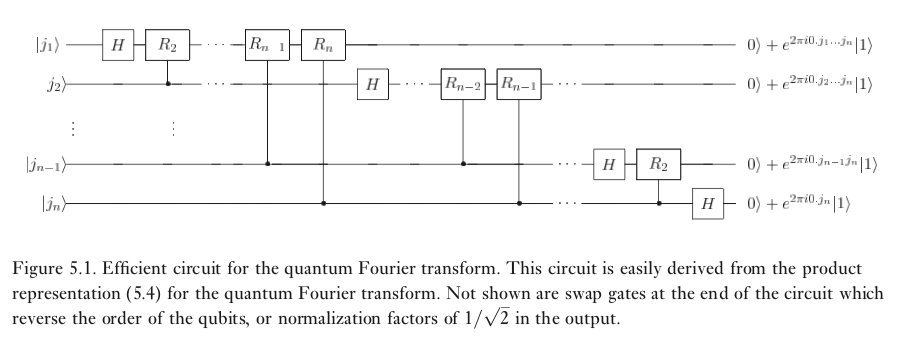
\includegraphics[width=\linewidth]{images/qfft.png}	
\end{figure}

Furthermore, the gate complexity is $O(n^2)$ as opposed to $O(n2^n)$, classically. 

\subsection{Quantum Phase Estimation Algorithm}\label{phase_estimation}

Suppose a unitary operator $U$ has an eigenvector $\ket{u}$ with eigenvalue $e^{2\pi i \phi}$, where the value of $\phi$ is unknown. 

\begin{figure}[H]
\centering
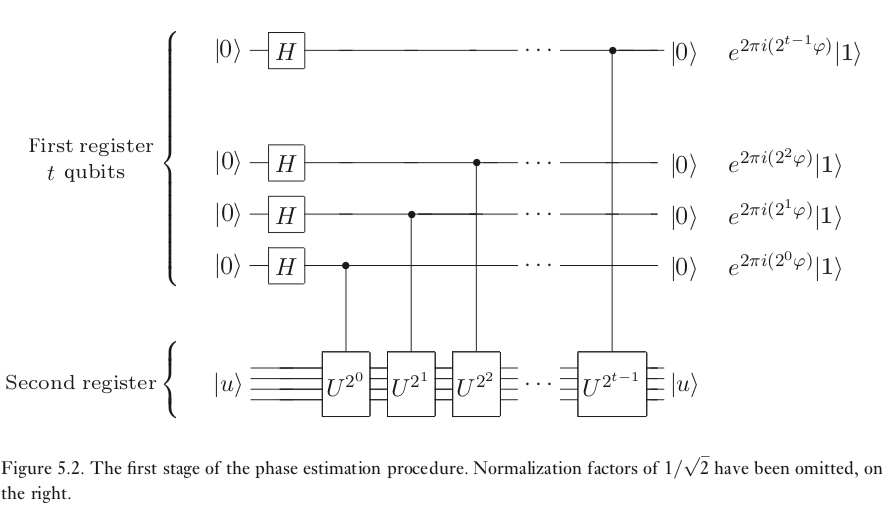
\includegraphics[width=\linewidth]{images/phase_estim.png}	
\end{figure}

Then, observe that the circuit above gives the state 

\begin{align*}
\frac{1}{2^t}(\ket{0} + e^{2 \pi i 0.\phi_t}\ket{1})(\ket{0} + e^{2 \pi i 0.\phi_{t-1}\phi_t}\ket{1})	\cdots (\ket{0} + e^{2 \pi i 0.\phi_1\phi_2\cdots\phi_t}\ket{1})	
\end{align*}

Hence, we can apply the inverse QFT and get the state $\ket{\phi_1 \cdots \phi_t}$, which is an approximation of $\phi$, whose accuracy is dependent on the size of $t$. 

Therefore, the complexity of this algorithm is essentially that of the inverse Fourier transform, $O(t^2)$. This assumes that each controlled-$U^{2^j}$ operation is given by an oracle, which may not hold in practice. Furthermore, we also assume that we can prepare $\ket{u}$ efficiently, which also may not hold in practice. Hence, we often require workarounds to these problems in our applications of Phase Estimation.

\begin{example} The effect of the sequence of controlled-$U$ operations like that in the figure is to take the state $\ket{j}\ket{u}$ to $\ket{j} U^j\ket{u}$. (Note that this does not depend on $\ket{u}$ being an eigenstate of $U$.)
\begin{proof}
	Consider an arbitrary $j$ in its binary representation $j_0j_1 \cdots j_{t-1}$ where $j_i \in \{ 0, 1\}$. Hence, for each $\ket{j_i}$, the control-$U$ acts on $\ket{j_i}\ket{u}$ such that $\ket{j_i}\ket{u} \mapsto \ket{j_i}U^{j_i 2^i}\ket{u}$. Therefore, the final state is given by
	
	\begin{align*}
	\ket{j_0 } \cdots \ket{j_{t-1}}U^{j_0 2^0} \cdots U^{j_{t-1} 2^{t-1}}\ket{u} &= \ket{j} U^{j_0 2^0} \cdots U^{j_{t-1} 2^{t-1}}\ket{u} \\
	&= \ket{j} U^{j_0 2^0 + j_{t-1} 2^{t-1}}\ket{u} \\
	&= \ket{j} U^{j}\ket{u}
	\end{align*}
\end{proof}
\end{example}

%\subsection{Order-Finding and Factoring}
%
\section{Quantum Search Algorithms}
\label{sec:search}
For more detail, we suggest Chapter 6 of \cite{nielsen2010quantum}.

\subsection{Grover's Algorithm and Amplitude Amplification}

Suppose we wish to search a space of elements of size $N$. Clearly this problem is $\Omega(N)$, classically. Rather than searching the elements directly, we can focus on "searching" their indices which are labelled $[ 0, N-1]$ by using an oracle. So, let $x \in [0, N-1]$ and $\ket{q}$ be an ancillary qubit. Define $f(x) = 1$ if the index is the index of the solution and $f(x) = 0$ otherwise. An oracle is a unitary operation, $O$, which acts on the computation basis as

\begin{align*}
\ket{x}\ket{q} \rightarrow^O \ket{x}\ket{q \oplus f(x)}
\end{align*}

Hence, if we let $\ket{q} = \frac{\ket{0}-\ket{1}}{\sqrt{2}} = \ket{-}$, then we can rewrite this transformation as

\begin{align*}
\ket{x}\ket{-} \rightarrow^O (-1)^{f(x)}\ket{x}\ket{-}	
\end{align*}

Grover \cite{grover1996fast} came up with a quantum algorithm that finds a solution with high probability using $O(\sqrt{N})$ oracle queries (which is known to be optimal on a quantum computer \cite{nielsen2010quantum}).

For $N = 2^n$, the grover iteration can be given by the linear transformation $G = (2\ket{\psi}\bra{\psi}-I)O$ where $\ket{\psi}$ is the equally weighted superposition of states. 

So, assuming that the number of solutions $M = 1$, Grover's algorithm essentially prepares $N$ qubits in state $\ket{\psi}\ket{-}$ and then applies $G$ for $\frac{\pi}{4}\sqrt{N}$ iterations. 

However, if the number of solutions $M \geq 1$ is unknown, then a variant, known as amplitude amplification \cite{brassard2002quantum}, can be used to find a solution in the solution subspace with high probability using $O(\sqrt{N/M})$ queries. 

\section{Quantum Information Theory}

Standard references on this matter are \cite{nielsen2010quantum} (we particularly use Chapter 12) and \cite{wilde2013quantum} (particularly Chapters 9 and 11).


\begin{definition}(Quantum Entropy)
Suppose that Alice prepares some quantum system $A$ in state $\rho_A$ (a density matrix in Hilbert space $\mathcal{H}_A$, equivalently $\rho_A \in D(\mathcal{H}_A)$). Then, the entropy $H(A)_\rho$  of the state is defined as follows

\begin{align}
	H(A)_\rho := -Tr(\rho_A \log \rho_A)
\end{align}
\end{definition}

\begin{definition}(Joint Quantum Entropy)
The joint quantum entropy $H(AB)_\rho$ of the density operator $\rho_{AB} \in D(\mathcal{H}_A \otimes \mathcal{H}_B)$ for a bipartite system $AB$ follows naturally from the definition of quantum entropy

\begin{align}
H(AB)_\rho := −Tr\{\rho_{AB}log \rho_{AB}\}
\end{align}
\end{definition}


\begin{definition}(Conditional Quantum Entropy)
Let $\rho_{AB} \in D(\mathcal{H}_A\otimes \mathcal{H}_B)$. The conditional quantum entropy $H(A\mid B)_\rho$ of $\rho_{AB}$ is equal to the difference of the joint quantum entropy $H(AB)_\rho$ and the marginal entropy $H(B)_\rho$:


\begin{align}
H(A\mid B)_\rho := H(AB)_\rho - H(B)_\rho	
\end{align}
\end{definition}

\begin{definition}
(Quantum Mutual Information) The quantum mutual information of a bipartite state $\rho_{AB} \in D(\mathcal{H}_A\otimes \mathcal{H}_B)$ is defined as follows:

\begin{align}
I(A: B)_\rho := H(A)_\rho + H(B)_\rho - H(AB)_\rho \\
= H(A)_\rho - H(A\mid B) \\
= H(B)_\rho - H(B \mid A) 
\end{align}

\end{definition}

\begin{proposition}
\label{prop:subadd-entropy}
(Subadditivity of Quantum Entropy)
The quantum entropy is sub-additive for a bipartite state $\rho_{AB}$:

\begin{align*}
H(A)_\rho + H(B)_\rho \geq H(AB)_\rho	
\end{align*}
\begin{proof}
Corollary 11.8.1 of \cite{wilde2013quantum}
\end{proof}
\end{proposition}

\begin{theorem}\label{thm:holevo}
(Holevo's Theorem)

Let $\{\rho_1, \rho_2, ..., \rho_n\}$ be a set of mixed states and let $\rho_X$ be one of these states drawn according to the probability distribution $P = \{p_1, p_2, \cdots , p_n\}$.

Then, for any measurement described by POVM elements ${E_Y}$ and performed on $ \rho =\sum _{X}p_{X}\rho _{X}$, the amount of accessible information about the variable $X$ knowing the outcome $Y$ of the measurement is bounded from above as follows:

$${ I(X:Y)\leq S(\rho )-\sum _{i}p_{i}S(\rho _{i})}$$ 

where $\rho =\sum _{i}p_{i}\rho _{i}$ and $ S(\cdot )$ is the von Neumann entropy.

The quantity on the right hand side of this inequality is called the Holevo information or Holevo $\chi$ quantity:

$$ \chi :=S(\rho )-\sum _{i}p_{i}S(\rho _{i})$$
\end{theorem}

\subsection{Pretty Good Measurement (PGM)}
\label{app:pgm}

Given a density matrix ensemble $\mathcal{E} = \{p_i, \sigma_i\}$ and a quantum state $\rho$ we are promised that $\rho$ is in state $\sigma_i$ with probability $p_i$. In the general case we have $i \in [m]$ and of course $\sum_{i=1}^m p_i = 1$. Our goal is then to successfully identify which of the $\sigma_i$ that our state $\rho$ is actually in. This is known as Quantum Hypothesis Testing. 

In some sense, thinking back to Holevo's Theorem (Theorem \ref{thm:holevo}), this is related to Bob attempting to access information transported from Alice that is given from the distribution above.

Hence, we perform a maximization with respect to both the probabilities on each state as well as with respect to any randomness that our approach employs. We then must choose a Quantum POVM $\{E_i\}$ that carries put a measurement and maximizes our probability of getting the state right.

So say we pick a POVM. Hence, we know that

\begin{align*}
\Pr(Success)= \sum_i p_i \Tr (\sigma_i E_i)
\end{align*}


So this is the quantity that we seek to maximize. 

We've shown above that the trace distance provides the solution for $m=2$. As it turns out for $m>2$ this is not an easy problem. However, PGM provides a sound approximation:

Intuitively, it might seem reasonable to simply choose 

$$E_i = p_i \sigma_i$$

Unfortunately, then, $\sum_i E_i \neq I$. Well, one case we may think about is if we can guarantee $\sigma_i$ is a the sum of pure states from an orthonormal basis. In which case, let $S = \sum_i \sigma_i$ and we choose 

$$E_i = S^{1/2} \sigma_i S^{1/2} $$ 

Then we have

$$
\tr(E_i \sigma_i) = \tr(\sigma_i) = 1
$$

by orthonormality. Inspired by this, define the PGM POVM to be 

$$E_i = S^{-1/2}p_i \sigma_i S^{-1/2}$$ 

for our original problem. Positive semidefiniteness is clear, so it remains to show that we have completeness

\begin{align*}
\sum_i E_i &= \sum_i S^{-1/2}p_i \sigma_i S^{-1/2}\\
&=  S^{-1/2} \sum_i p_i \sigma_i S^{-1/2} \\
&= S^{-1/2} S S^{-1/2} = I
\end{align*}

\begin{theorem}
Let $\Pr_{opt}(\mathcal{E})$ by the optimal success probability for our 	quantum hypothesis testing problem. Define $\Pr_{PGM}(\mathcal{E})$ to be the average success probability using the PGM POVM. Then,

\begin{align*}
Pr_{opt}(\mathcal{E})^2 \leq Pr_{PGM}(\mathcal{E}) \leq 	Pr_{opt}(\mathcal{E})
\end{align*}

\end{theorem}

\subsection{Trace Distance}

\begin{definition}
Trace Distance

The trace distance $T(\cdot , \cdot)$ is a metric on the space of density operators and gives a measure of distinguishability between states. In particular, let $\rho, \sigma$ be density operators,

\begin{align*}
	T(\rho, \sigma) &= \frac{1}{2} \Tr [\sqrt{(\rho - \sigma)^2}] \\
	&= \frac{1}{2} \sum_i |\lambda_i|
\end{align*}

where $\lambda_i$ are the eigenvalues of Hermitian $\rho - \sigma$.

Hence, it is simply the trace norm of the positivization of the difference of matrices.

\end{definition}

\begin{lemma}
\label{lem:nc97}
For any states $\rho, \sigma$ one may write $\rho - \sigma = Q - S$ where $Q$ and $S$ are positive operators with support on orthogonal vector spaces	(Exercise 9.7 \cite{nielsen2010quantum})
\end{lemma}

\begin{proof}
$\rho, \sigma$ are p.s.d operators. Hence, $\rho - \sigma$ is Hermitian, so we can write $\rho - \sigma = \sum_i \lambda_i \ket{u_i}\bra{u_i}$ where $\{ u_i \}$ is an orthonormal basis of the Hilbert space, by spectral theorem. Now, we can decompose the eigenbasis into positive and negative components. Then, $\rho - \sigma = \sum_i \lambda^+_i \ket{u_i}\bra{u_i} + \sum_j \lambda^-_j\ket{u_j}\bra{u_j}$ where $\lambda^+_i >0, \lambda^-_j < 0$. Since, each component partitions the vector space (other than at the additive identity) by the orthogonality condition, this is a direct sum.
\end{proof}


\begin{lemma}
\label{lem:holder}
	(Holder's Inequality for matrices)
	
	Given Hermitian $A, B$ and $p,q \in [1, \infty]$ such that $\frac{1}{p}+\frac{1}{q} = 1$,
	
	\begin{align*}
	\tr(AB) \leq \|A\|_p\|B\|_q	
	\end{align*}
\end{lemma}


\begin{proposition}
The maximum probability of distinguishing between two states with an optimal measurement is given by

\begin{align*}
	1/2[1 + T(\rho_1, \rho_2)]
\end{align*}
	
\end{proposition}
\begin{proof}
Say that we have the "worst-case" (equally mixed) ensemble $\{ (1/2, \rho_1), (1/2, \rho_2)\}$. We seek to define a POVM $\{E_1, E_2 \}$ where $E_1$ indicates $\rho_1$ and similarly for $\rho_2$. hence the probability of success is given by

\begin{align*}
\Pr_{\max} &= \max_{E_1, E_2} 1/2 \Tr[E_1\rho_1] + 1/2 \Tr[E_2\rho_2] \\
&= \max_{E_1, E_2} 1/2[1/2 \Tr[(E_1+E_2)(\rho_1 + \rho_2)] + 1/2 \Tr[(E_1 - E_2)(\rho_1 - \rho_2)]] \tag{linearity of trace}\\
&= \max_{E_1, E_2} 1/2[1/2 \Tr[(\rho_1 + \rho_2)] + 1/2 \Tr[(E_1 - E_2)(\rho_1 - \rho_2)]] \tag{Completeness of POVM} \\
&= \max_{E_1, E_2} 1/2[1 + 1/2 \Tr[(E_1 - E_2)(\rho_1 - \rho_2)]] \tag{trace of density operator is 1}
\end{align*}

Hence, Holder's inequality says that 

\begin{align*}
\Tr[(E_1 - E_2)(\rho_1 - \rho_2)] &\leq \|E_1 - E_2 \|_\infty \|\rho_1 - \rho_2 \|_1 \\
&\leq \|\rho_1 - \rho_2 \|_1
\end{align*}

as desired. The first inequality follows by choosing $p = \infty, q = 1$ in Lemma \ref{lem:holder}. The second inequality follows from $E_1, E_2$ being projector matrices and so the spectra of each satisfies $0 \leq \lambda(E_i) \leq 1$.

We can achieve this upper bound by , the optimal projection $E_1 - E_2$ is choosing $E_1$ to orthogonally project onto the positive eigenspace $Q$ of $(p_1\rho_1 - p_2\rho_2)$ and $E_2$ the negative eigenspace $S$ (we can do so by Lemma \ref{lem:nc97}). Write that the eigenvectors which span $P$ have eigenvalues $\{ \lambda_i \}_{1 \leq i \leq m}$ and $Q$ with $\{\mu_i \}_{1 \leq i \leq m'}$. Then, 

\begin{align*}
1/2\Tr[(E_1 - E_2)(\rho_1 - \rho_2)] &= 1/2\Tr[E_1(\rho_1 - \rho_2)] - \Tr[E_2(\rho_1 - \rho_2)] \\
&= 1/2 \sum_i \lambda_i - 1/2 \sum_i \mu_i = 1/2 \| \rho_1 - \rho_2 \|_1
\end{align*}

as desired\footnote{We did implicitly assume that $E_1 + E_2 = I$ where we could've had an additional indeterminate $E_3$. However, the proof would still follow in any case (\cite{nielsen2010quantum}).}.
\end{proof}


\begin{corollary}
\label{cor:distinguish-two-pure-states}
Consider attempting to distinguish two pure states $\ket{\psi_0}, \ket{\psi_1}$. Then, we will distinguish correctly with probability at most $1/2[1 + \sqrt{1 - |\bra{\psi_0}\ket{\psi_1}|^2}]$.

Equivalently, if we can distinguish between the two states w.p. $1 - \delta$, then $|\bra{\psi_0}\ket{\psi_1}| \leq 2\sqrt{\delta(1-\delta)}$. 	
\end{corollary}

\begin{proof}
Applying the previous Lemma, we have maximum probability

\begin{align*}
1/2[1 + T(\ket{\psi_0}\bra{\psi_0}, \ket{\psi_1}\bra{\psi_1}	)]
\end{align*}

So, write $\ket{\psi_1} = \cos(\theta) \ket{\psi_0} + e^{i\phi}\sin(\theta)\ket{\psi_0^\perp}$. Hence,

\begin{align*}
\ket{\psi_1}\bra{\psi_1}	 &= \cos^2(\theta) \ket{\psi_0}\bra{\psi_0} + \sin^2(\theta)\ket{\psi_0^\perp}\bra{\psi_0^\perp}
+ e^{i\phi}\cos(\theta)\sin(\theta)\ket{\psi_0^\perp}\bra{\psi_0} + e^{-i\phi}\cos(\theta)\sin(\theta)\ket{\psi_0}\bra{\psi_0^\perp}
\end{align*}

Since trace is basis-independent, we can write $\ket{\psi_0}\bra{\psi_0} - \ket{\psi_1}\bra{\psi_1}$ in the above used orthogonal basis. This gives us characteristic polynomial

\begin{align*}
	0 &= (1-\cos^2(\theta) - \lambda)(-\sin^2(\theta) - \lambda) - \cos^2(\theta)\sin^2(\theta)\\
	&= (\sin^2(\theta) - \lambda)(-\sin^2(\theta) - \lambda) - \cos^2(\theta)\sin^2(\theta) \\
	&= -\sin^4(\theta) + \lambda^2 - \cos^2(\theta)\sin^2(\theta) \\
	&= -\sin^2(\theta) + \lambda^2
\end{align*}

 So, $\lambda = \pm |\sin(\theta)|$. Therefore, since the trace distance is the absolute sum of the eigenvalues of this difference, 

\begin{align*}
T(\ket{\psi_0}\bra{\psi_0}, \ket{\psi_1}\bra{\psi_1}	) &= 2|\sin(\theta)|
\end{align*}

and indeed 

\begin{align*}
|\bra{\psi_0}\ket{\psi_1}|^2 &= |\cos(\theta)|^2\\
\implies \sqrt{1 - |\bra{\psi_0}\ket{\psi_1}|^2} &= |\sin(\theta)|
\end{align*}

as desired.
\end{proof}


\begin{lemma}
\label{lem:psd-trace}
Let $A, B, C$ by symmetric $d \times d$ matrices satisfying $A \succeq 0$ and $B \preceq C$. Hence, $\Tr(AB) \leq \Tr(AC)$

\begin{proof}
	Write $A$ in its spectral decomposition $A = \sum \lambda_i \ket{i}\bra{i}$, invoking Spectral Theorem (\ref{thm:spec}). Hence,
	
	\begin{align*}
		\Tr(AB) &= \Tr(\sum \lambda_i \ket{i}\bra{i} B)\\
		&= \sum \lambda_i \Tr(\ket{i}\bra{i} B) \tag{linearity of trace}\\
		&= \sum \lambda_i \Tr(\bra{i} B \ket{i}) \tag{cyclic property of trace}\\
		&\leq \sum \lambda_i \Tr(\bra{i} C \ket{i})\\
		&= \sum \lambda_i \Tr(\ket{i}\bra{i} C) = \Tr(\sum \lambda_i \ket{i}\bra{i} C) = \Tr(AC)
	\end{align*}
\end{proof}
\end{lemma}

\begin{corollary}
\label{cor:psd-tr-norm-ineq}
If $A, B \succeq 0$, then $\Tr(AB) \leq \Vert B \Vert_2 \Tr(A)$

\begin{proof}
Note that the singular values of $B$ coincide with the eigenvalues of $B$ since $B^\dag B = B^2$ and $B \succeq 0$ $\implies$ $\lambda_i(B) \geq 0$, $\forall i$. So, let $C = \Vert B \Vert_2 I$ which then trivially satisfies $\lambda_i(C) = \lambda_{\max}(B)$, $\forall i$ since $C$ is the diagonal matrix with diagonal values all equal to $\lambda_{\max}(B)$. Therefore, $B \preceq C$. So, we can simply apply \ref{lem:psd-trace} above,

\begin{align*}
\Tr(AB) &\leq \Tr(AC) \\
&= \Tr\big(A \Vert B \Vert_2 I\big)\\
&= \Vert B \Vert_2 \Tr(A)
\end{align*}
\end{proof}
\end{corollary}

\end{document}